% !TEX root = ../CSS-OS.tex

\chapter{约束}
本章主要讨论有哪些因素会影响到望远镜的曝光过程。这些因素可以分为两大类:1)光学设施的硬件约束;
2)天文观测条件。另外还包括南大西洋异常区对仪器的影响,轨道维持,中继卫星通信,停靠维护。

\MT{有必要花一些时间对这些条件建立合理的物理模型,从而改进具体的代码实现(尽量减少判断语句的使用)。}



\section{光学设施硬件约束}

\subsection{能源因素}

\subsubsection{早期约束条件}
太阳帆板与太阳的位置关系,需要考虑卫星所在的位置,当卫星所在的位置为阴影区,帆板与太阳的位置
关系不需要考虑;当卫星所在的区域为阳照区,需要考虑帆板与太阳的位置关系,以保障能源的供应,帆板
面的法线与太阳的夹角在[-25\textdegree,25\textdegree]之间。在此基础上还需要考虑如下
的能源平衡条件:

\begin{table}[h!]
\renewcommand{\arraystretch}{1.5}
\centering
%\begin{tabular}{|c|c|}
\begin{tabular}{m{.45\textwidth}<{\centering}| m{.45\textwidth}<{\centering}}
\toprule
 {\large 初期 (条件2)} & {\large 末期 (条件1)} \\
\hline
阳照区帆板法线与太阳矢量夹角5\textdegree-10\textdegree 的观测姿态+转动总时间不大于48分钟 &
阳照区帆板法线与太阳矢量夹角5\textdegree-10\textdegree 的观测姿态+转动总时间不大于31分钟 \\
\hline
阳照区帆板法线与太阳矢量夹角10\textdegree-15\textdegree 的观测姿态+转动总时间不大于30分钟 &
阳照区帆板法线与太阳矢量夹角10\textdegree-15\textdegree 的观测姿态+转动总时间不大于16分钟 \\
\hline
阳照区帆板法线与太阳矢量夹角15\textdegree-20\textdegree 的观测姿态+转动总时间不大于17分钟 &
阳照区帆板法线与太阳矢量夹角15\textdegree-20\textdegree 的观测姿态+转动总时间不大于10分钟 \\
\hline
阳照区帆板法线与太阳矢量夹角20\textdegree-25\textdegree 的观测姿态+转动总时间不大于10分钟 &
阳照区帆板法线与太阳矢量夹角20\textdegree-25\textdegree 的观测姿态+转动总时间不大于10分钟,
则下一轨阳照区的观测和机动必须保证帆板法线对日 \\
\hline
阳照区帆板法线与太阳矢量夹角20\textdegree-25\textdegree 的观测姿态+转动总时间10-15分钟,
则下一轨阳照区的观测和机动必须保证帆板法线对日 &
阳照区非观测且非姿态机动保证法线对日 \\
\hline
阳照区非观测且非姿态机动保证法线对日 & \\
%\hline
\bottomrule
\end{tabular}
\caption{能源平衡条件}
\label{tab:energy_balance}
\end{table}

张鑫通过建立如下的一个数学模型来反推出不同角度时帆板的发电功率。假设每轨的时间为92分钟,每轨
中阳照区时间为57分钟,阴影区时间为35分钟,并假设设备的整体功耗为1J/s。根据该假设,可以从条件1
(见表~\ref{tab:energy_balance})可以列出如下能源平衡方程:
\begin{eqnarray}
P_1\times 31 + P_0\times 26 &=& 92\times 1,\\
P_2\times 16 + P_0\times 41 &=& 92\times 1,\\
P_3\times 10 + P_0\times 47 &=& 92\times 1,\\
P_4\times 10 + P_0\times 104 &=& 92\times 1\times 2,
\end{eqnarray}
以及
\begin{eqnarray}
P_1 &=& \cos 5\textdegree \times \cos 5\textdegree \times P_0,\\
P_2 &=& \cos 10\textdegree \times \cos 10\textdegree \times P_0,\\
P_3 &=& \cos 15\textdegree \times \cos 15\textdegree \times P_0,\\
P_4 &=& \cos 20\textdegree \times \cos 20\textdegree \times P_0.
\end{eqnarray}
其中$P_i$表示帆板在不同角度下的发电功率($i=0,1,2,3,4$分别对应于
$0\textdegree\sim 5\textdegree$,
$5\textdegree\sim 10\textdegree$,
$10\textdegree\sim 15\textdegree$,
$15\textdegree\sim 20\textdegree$,
和$20\textdegree\sim 25\textdegree$)。

\RT{{\heiti 一点思考:} 张鑫在这一块的处理似乎有点问题,他得到的$P_i$的值,似乎不满足初始和末期的
一个$7\%$的差异。}

\subsubsection{动态计算能源水平}
太阳能帆板以及发电效率的相关信息见~\ref{chap_internal}的内容。

\subsection{CMG温度影响}

\begin{table}[h!]
\renewcommand{\arraystretch}{1.5}
\centering
%\begin{tabular}{|c|c|}
\begin{tabular}{m{.4\textwidth}<{\centering}| m{.2\textwidth}<{\centering}| m{.2\textwidth}<{\centering}}
\toprule
\multirow{4}{*} & 姿态机动角度(\textdegree) & 单轨允许机动次数 \\ \cline{2-3}
				& 5-10 & 29 \\ \cline{2-3}
				& 10-20 & 19 \\ \cline{2-3}
				& 20-35 & 13 \\ \cline{2-3}
CMG工况温度对机动次数的影响 & 35-45 & 10 \\ \cline{2-3}
\multirow{4}{*} & 45-75 & 6 \\ \cline{2-3}
				& 75-90 & 5 \\ \cline{2-3}
				& 90-135 & 3 \\ \cline{2-3}
				& 135-180 & 2 \\ 
\bottomrule
\end{tabular}
\caption{CMG温度约束对机动角度、次数的限制。}
\label{default}
\end{table}

\section{天文观测条件}

\subsection{太阳}
在曝光的过程中,望远镜的视轴方向与太阳方位矢量的夹角不得小于50\textdegree。

\subsection{月球}
在曝光的过程中,望远镜的视轴方向与月球方位矢量的夹角不得小于40\textdegree。该规避角(40\textdegree)是假设月球处于满月
的时候估算出来的(需要进一步确认)。


\subsection{地球遮挡与反照}
地球对近地轨道望远镜观测方向有较大的影响。首先,地球所遮挡的方向无法观测。其次,地球反照光可对
望远镜造成很高的背景噪声,大大降低观测效率。地球遮挡与反照可以统一考虑,做如下要求:望远镜观测
方向与地球亮边夹角$\ge70$\textdegree,望远镜观测方向与地球暗边夹角$\ge30$\textdegree。

\BT{是否需要进一步考虑地球大气折射的因素,并以此进一步得到更加严格的夹角的限制条件?}

\subsection{黄道光}

\subsection{银盘}
包括银河系内的亮星的影响


\section{南大西洋磁场异常区}
南大西洋磁场异常区(SAA)为范艾伦辐射带接近地球表面的区域,大量的太阳粒子落在该区域,对于低轨飞行器有
很大的影响。通过该区域上空时,为了避免异常运作,望远镜必须关机\footnote{但是其他组件,比如制冷、发电装
置持续工作。}。\BT{张鑫:这一部分已经写好函数可以获取某一位置的粒子数目进行判断。}

\begin{figure}
\centering
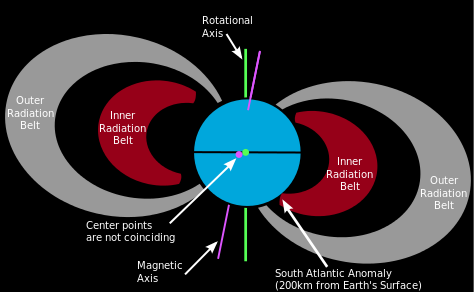
\includegraphics[width=0.6\textwidth,angle=0]{figs/South_Atlantic_Anomaly.png}
\caption{南大西洋磁场异常区的成因。A cross-sectional view of the Van Allen radiation belts, noting
the point where the South Atlantic Anomaly occurs. The figure is taken
from:~\url{https://en.wikipedia.org/wiki/South_Atlantic_Anomaly}.}
\label{fig:saad1}
\end{figure}

\begin{figure}
\centering
\includegraphics[width=0.65\textwidth,angle=-90]{figs/saad.ps}
\caption{南大西洋磁场异常区。The South Atlantic Anomaly (SAA, the large red area in the image)
is a dip in the Earth's magnetic field which allows cosmic rays, and charged particles to
reach lower into the atmosphere. This interferes with communication with satellites, aircraft,
and the Space Shuttle. While there are theories as to why this occurs, the geologic origin
is not yet known. The figure is taken
from:~\url{https://heasarc.gsfc.nasa.gov/docs/rosat/gallery/misc_saad.html}.}
\label{fig:saad2}
\end{figure}

\BT{后续优化的时候,可以将SAA区域的信息整合到预先计算好的卫星轨道数据中去,这样一来就免去了模拟的
过程中再去计算和判断望远镜是否处于SAA区域。}

\subsection{3月22日笔记}
今天在读张鑫的程序时看到一段代码,其中有一个while循环,退出该循环的条件是望远镜不在SAA区域。
原先文档里提到在SAA区域上空时,望远镜必需关机。而我原先以为是整个望远镜模块都要关机,但实际上像
发电装置、制冷设备等都一直在工作。



